\documentclass[french, a4paper, 12pt, titlepage]{article}
%% Peut remplacer "article" par "scrartcl" %%

\usepackage[french]{babel}
\usepackage{a4wide}
%\usepackage[top=2cm, bottom=2cm, left=2cm, right=2cm]{geometry}
\raggedbottom % prevents vertical white space on pages that cannot be filled properly

\usepackage{hyperref}
\hypersetup{
	colorlinks=true,       	% false: boxed links; true: colored links
	linkcolor=black,          	% color of internal links
	urlcolor=blue,           	% color of external links
	citecolor=grey
}

\usepackage[T1]{fontenc}
%\usepackage{fourier}
%\usepackage{utopia}
%\usepackage{palatino}

\usepackage{lmodern}
%% ajouter fonte petite capitale grasse à lmodern avec celle de computer modern %%
\rmfamily
\DeclareFontShape{T1}{lmr}{b}{sc}{<->ssub*cmr/bx/sc}{}
\DeclareFontShape{T1}{lmr}{bx}{sc}{<->ssub*cmr/bx/sc}{}
%% /ajout %%
\usepackage{wrapfig}

%\usepackage[a4paper]{geometry} % marges plus petites que a4paper standard
\usepackage{listings} % insérer code source
\lstloadlanguages{sh,bash,awk,make}
%\usepackage{algorithm} % algorithmique
%\usepackage{algorithmic}
\usepackage{url}
\usepackage[usenames, dvipsnames]{color} % couleurs (nombre de base étendu)
\usepackage{graphicx} % insérer images
\usepackage[utf8]{inputenc}
\usepackage{amsmath}
\usepackage{amsfonts}
\usepackage{amssymb}
\usepackage{amsthm}
\usepackage{multicol}
\definecolor{grey}{rgb}{0.96,0.96,0.96}
\definecolor{grey2}{rgb}{0.3,0.3,0.3}

%% Define listings params %%
\lstset{
%	numbers=left,
	language=bash,
	tabsize=4,
	frame=single, % cadre autour du code
	breaklines=true, % autorise couper ligne trop longue
	basicstyle=\small\ttfamily,
	numberstyle=\scriptsize\ttfamily,
	backgroundcolor=\color{grey},
	showstringspaces=false,
	keywordstyle=\color{OliveGreen},
	stringstyle=\color{BrickRed},
	commentstyle=\color{grey2}\it,
	stepnumber=1 % numérote toute les x lignes
}
% listing utf8 fr %
\lstset{%
	inputencoding=utf8,
	extendedchars=true,
	literate=
		{é}{{\'{e}}}1
		{è}{{\`{e}}}1
		{ê}{{\^{e}}}1
		{ë}{{\¨{e}}}1
		{û}{{\^{u}}}1
		{ù}{{\`{u}}}1
		{â}{{\^{a}}}1
		{à}{{\`{a}}}1
		{î}{{\^{i}}}1
		{ç}{{\c{c}}}1
		{Ç}{{\c{C}}}1
		{É}{{\'{E}}}1
		{Ê}{{\^{E}}}1
		{À}{{\`{A}}}1
		{Â}{{\^{A}}}1
		{Î}{{\^{I}}}1
}
%% /Define listings params %%

%% Francisation des algorithmes
%\renewcommand{\algorithmicrequire} {\textbf{\textsc{Entrées:}}}
%\renewcommand{\algorithmicensure}  {\textbf{\textsc{Sorties:}}}
%\renewcommand{\algorithmicwhile}   {\textbf{tant que}}
%\renewcommand{\algorithmicdo}      {\textbf{faire}}
%\renewcommand{\algorithmicendwhile}{\textbf{fin tant que}}
%\renewcommand{\algorithmicend}     {\textbf{fin}}
%\renewcommand{\algorithmicif}      {\textbf{si}}
%\renewcommand{\algorithmicendif}   {\textbf{fin si}}
%\renewcommand{\algorithmicelse}    {\textbf{sinon}}
%\renewcommand{\algorithmicthen}    {\textbf{alors}}
%\renewcommand{\algorithmicfor}     {\textbf{pour}}
%\renewcommand{\algorithmicforall}  {\textbf{pour tout}}
%\renewcommand{\algorithmicdo}      {\textbf{faire}}
%\renewcommand{\algorithmicendfor}  {\textbf{fin pour}}
%\renewcommand{\algorithmicloop}    {\textbf{boucler}}
%\renewcommand{\algorithmicendloop} {\textbf{fin boucle}}
%\renewcommand{\algorithmicrepeat}  {\textbf{répéter}}
%\renewcommand{\algorithmicuntil}   {\textbf{jusqu'à}}
%\renewcommand{\algorithmiccomment} {\STATE //}
%\newcommand{\BEGIN}{\STATE \fbox{Début}}
%\newcommand{\END}{\STATE \fbox{Fin}}
%\floatname{algorithm}{Algorithme}
%% /francisation des algorithmes

\renewcommand{\qedsymbol}{}

\newcommand{\petit}[1]{
	\medskip \noindent
	\begin{small}
	#1)
	\end{small}
}

\begin{document}

\title{Introduction aux commandes shell (Linux) basique}
\author{Club*Nix}
\date{Compilé le \today}

\maketitle
%% Laisse page blanche pour verso page de garde %%

\vfill
\pagebreak

%\tableofcontents
\newpage
\strut\thispagestyle{empty}
\vfill
\pagebreak
\tableofcontents
\strut\thispagestyle{empty}
%\setcounter{page}{0}
\newpage
\setcounter{page}{1}

\section{Presentation d'un environnement GNU/Linux}
Le projet \textit{GNU/Linux} commence en 1983 lorsque Richard Stallman commence le projet GNU, proposant de développer un ensemble de logiciels libres, mais ce n'est qu'en 1992 après des avoir fini la plupart des outils essentiels (gcc, emacs, les cores utils ...) sauf leurs kernel \textit{Hurd} que Linus en propose un, \textit{Linux}, et permet de lancer un système exempt de tout logiciel propriétaire.
A l'heure actuelle, GNU/Linux est essentiellement utilisé en tant que serveur et par quelques geeks qui souhaitent avoir un contrôle sur ce qu'ils exécutent sur leur ordinateur. La philosophie initiale de Stallman commence à toucher un plus grand public (avec notamment les administrations qui commencent à virer tous les produits Micro\$oft).

Pour la petite histoire, le logo de Linux n'est pas un pingouin mais un \textbf{manchot}, plus exactement un manchot pygmée \url{https://fr.wikipedia.org/wiki/Manchot_pygmée}. Linus est en effet revenu avec cette idée de mascotte après s'être fait mordre lors d'un voyage en Australie par cette même espèce de manchot et coupa court à la discussion qui se portait sur un requin.

\section{Qu'est-ce que le Shell}
Le Shell, ou coquillage correspond à l'interpréteur de commande utilisé à l'intérieur de votre terminal.
C'est l'interface minimale entre l'utilisateur et le système d'exploitation.
Il en existe de toutes sortes (bash, tcsh, sh, ksh, zsh \dots). Tous permettent d'exécuter des commandes, programmes <insert text here>.
Dans le monde réel, \emph{bash} est l'interpréteur le plus courant, cependant pour quelque raison obscure, vous commencerez par défaut votre aventure à l'ESIEE avec \emph{tcsh}.
Très peu convivial, nous supposerons pour la suite que vous utilisez bash (vous pouvez lancer le shell \emph{bash} à l'intérieur de \emph{tcsh} en tapant la commande <<~bash~>> à l'affichage de votre \emph{prompt}).
Votre terminal est donc composé d'une fenêtre, permettant d'afficher un historique de commandes, de menus pour configurer les couleurs, la police\dots, et enfin du \emph{shell}, l'interpréteur qui est lancé automatiquement.
Ce que vous pouvez voir à partir de là est une ligne ressemblant à ceci :
\begin{lstlisting}
club@nix ~ $
\end{lstlisting}
%PS1="\[\033[01;32m\]club@nix\[\033[01;34m\] \w \$\[\033[00m\] "
\begin{center}
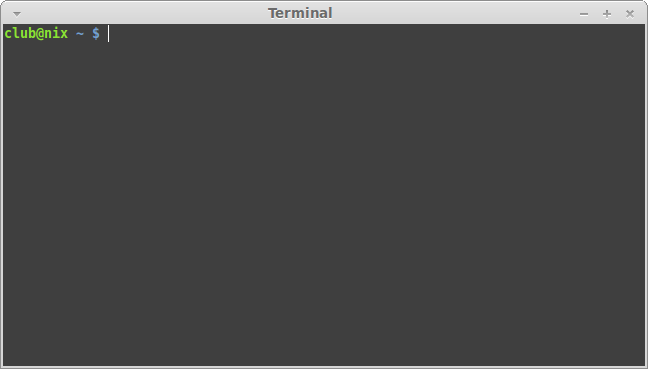
\includegraphics[scale=0.42]{Images/terminal}
\end{center}
Vous avez donc un affichage d'un certain nombre d'informations à travers votre \emph{prompt}.
\begin{enumerate}
\item[club@nix] correspond à votre login (nom d'utilisateur, ici <<~club~>>) suivi du nom de la machine (ici <<~nix~>>) sur laquelle vous vous trouvez, le tout est séparé par le caractère <<~@~>>.
\item[$\sim$] Vient ensuite votre dossier courant suivit du caractère "\$" (le dossier $\sim$ est un raccourci vers \emph{/home/club/}).
\item[\$] Enfin la ligne de commande, vous permettant de taper des... commandes. Le dollar signifie juste que vous avez la main (vous pouvez tapez vos commandes).
\end{enumerate}

\section{Notation}
\begin{enumerate}
\item[\^{}] correspond à la touche <<~\emph{Ctrl}~>>, \^{}C, signfie donc qu'il faut appuyer en même temps sur la touche "Ctrl" et C (deux touches sont enfoncées).
\item [<super>] correspond à la touche "super" honteusement surmontée par un logo windows sur la plupart des claviers.
\item [M-] correspond à la touche "Meta", le "alt" à côté de la touche espace.
\end{enumerate}

\newpage
\section{Commandes Basiques (débutant)}
\noindent Voici votre première expérience du terminal!\\
Pour lancer la bête, vous pouvez tester les différentes solutions suivantes:
\begin{itemize}
\item Menu -> barre de recherche -> "terminal" (ou "konsole" ou "gnome-terminal" ou "xfterm4" ou "xfce4-terminal")
\item Alt + f2 -> taper "terminal"
\item application -> accessoires -> terminal
\item <super>  -> taper "terminal"
\item \^{}M-t
\item sinon le logo à rechercher ressemble à ça:  
\includegraphics[scale=0.7]{Images/termIcon}
\end{itemize}
Il peut vous faire peur et picoter les yeux mais n'ayez crainte. Tout d'abord commençons par ce picotement des yeux, en faisant un clic droit et en allant dans profils, préférences du profil vous pourrez changer la couleur pour quelque chose de moins agressif pour vos yeux, "blanc sur noir" ou "vert sur noir" (pour les plus geeks d'entre vous) plusieurs choses peuvent être configurées, je vous laisse les découvrir.

Enfin, notez que vous trouverez avec ce document un dossier \emph{Exemple} contenant les exemples cités.

\subsection{Raccourcis utiles}
\begin{description}
\item[Entrée]: la plus importante, lance votre commande
\item[Flêche haut]: naviguer dans l'historique des commandes. Vous pourrez ainsi gagner du temps et éviter de retaper tojours la même chose
\item[Tab]: touche de complétion. Vous permet de taper les quelques premières lettres de votre commande, puis de les compléter. Si rien ne s'affiche la première fois que vous appuyez sur la touche, c'est qu'il existe plusieurs possibilités de complétion. Une seconde pression vous permettra d'afficher toutes les complétions possibles.
\item[Ctrl + Z]: pause la commande en cours.
\item[Ctrl + C]: arrête la commande en cours, annule l'opération en cours et recommence avec une nouvelle ligne. Très utile si vous voulez annuler l'exécution d'un programme qui boucle de manière infinie, ou si vous vous rendez compte que vous êtes en train d'écrire n'importe quoi.
\item[Ctrl+L]: nettoie l'écran
\end{description}

\subsection{Liste de commandes (formulaire)}
\begin{description}
\item[cat] \emph{con\textbf{cat}enate files} affiche un fichier sur l'entrée standard.
  \begin{lstlisting}
cat plop.txt
  \end{lstlisting}
\item[ls] \emph{\textbf{l}i\textbf{s}t directory contents} permet d'afficher le contenu d'un répertoire.
  \begin{lstlisting}
ls -lah
  \end{lstlisting}
\item[cd] \emph{\textbf{c}hange \textbf{d}irectory} permet de naviguer à travers les répertoires.
  \begin{lstlisting}
cd /usr/src/linux
  \end{lstlisting}
\item[cp] \emph{\textbf{c}o\textbf{p}y files} copie un fichier.
  \begin{lstlisting}
# Pour un fichier
cp /tmp/plop.txt /home/trax/

# Pour un  répertoire
cp -r /tmp/foo /home/trax
  \end{lstlisting}
\item[mv] \emph{\textbf{m}o\textbf{v}e file} déplace un fichier.
  \begin{lstlisting}
mv /tmp/foo /home/trax
  \end{lstlisting}
\item[./<exec>] lance le script/programme \emph{<exec>}
  \begin{lstlisting}
# Pour lancer a.out
./a.out
  \end{lstlisting}
\item[man] \emph{reference \textbf{man}uals} affiche un manuel sur une commande, fonction, bibliothèque (essayez "man man").
  \begin{lstlisting}
# Manuel d'utilisation de la command man
man man

# Fail
man woman
  \end{lstlisting}
\end{description}

\subsection{Details des commandes}
\subsection{Cat}
\subsubsection{Description}
\emph{Cat} est une commande permettant d'afficher du texte sur l'entrée standard.
Elle prend en entrée un fichier: texte, code source, script... pour l'afficher directement sur le terminal.

Attention toutefois : lors de son utilisation sur un fichier binaire, la commande s'exécutera bien. Cependant, le contenu du fichier est souvent trop gros pour votre terminal, et la suite de caracteres ASCII aléatoires à laquelle il correspond cassera votre terminal lorsque cat essaiera de l'afficher.
Si par inadvertance cela vous arrivait, vous pouvez toujours essayer de taper "reset" pour rétablir votre shell (il n'y a pas d'inquiétude à avoir si vous ne voyez pas la commande "reset" s'afficher, les caractères tapés sont bien pris en compte).


\subsubsection{Exemple d'utilisation}

\begin{lstlisting}
$ls
chaton.txt chat.c poulpe.exe
$cat chat.c
#include <stdio.h>

int main(){
	printf("oh, un chat!");
 return 0;
}
$
\end{lstlisting}

\subsection{ls}
\subsubsection*{Description}

\paragraph{} \texttt{ls} liste les fichiers et dossiers présents dans le
répertoire courant. Il prend en paramètre un dossier dont on veut lister les
fichiers. Sans paramètre cette commande liste les fichiers contenus dans le
répertoire courant. Il existe plusieurs options utiles à cette commande, comme
\texttt{-l} qui donne des informations détaillées sur les fichiers. Une autre
option utile est \texttt{----color} qui permet d'obtenir des indications sur
les fichiers en colorant leurs noms; les fichiers exécutables
deviennent vert, les dossiers bleus\ldots

\subsubsection*{Exemple d'utilisation}
\begin{lstlisting}
$ ls
Dossier/
$ ls Dossier/
texte.txt code.c image.png
$ ls -l Dossier/
total 20
-rw-r--r-- 1 club user    13 déc.   6 01:32 texte.txt
-rwxr-xr-x 1 club user 10019 déc.   6 01:33 image.png
-rw-r--r-- 1 club user   301 déc.   6 01:33 code.c
\end{lstlisting}

\paragraph{} On voit que l'option \texttt{-l} affiche plein d'informations
utiles. La première colonne indique les droits sur le fichier, que l'on
expliquera après, la troisième colonne avec \texttt{club} indique le
propriétaire du fichier (donc le propriétaire est l'utilisateur \texttt{club}).
La quatrième colonne représente le groupe propriétaire du fichier. Dans cet
exemple, le groupe propriétaire est le groupe \texttt{user}, qui est le groupe
des utilisateurs normaux. La cinquième colonne est la taille du fichier en
octets. Attention, la taille affichée par \texttt{ls -l} pour les dossiers ne
correspond pas à la taille de tous les sous-fichiers, et sous-dossiers. La
sixième colonne est la date de dernière modification du fichier (à savoir ici
le 6 décembre 1h33).

\paragraph{} Pour la première colonne, il faut savoir que les fichiers sous
GNU/Linux ont trois permissions principales: le droit de lecture (représenté
par \texttt{r} pour \emph{read}), le droit d'écriture (représenté par
\texttt{w} pour \emph{write}) et le droit d'exécution (représenté par
\texttt{x} pour \emph{eXecute}).

\paragraph{} La première lettre de cette colonne correspond au type de fichier.
Si par exemple, il s'agit d'un dossier, on verra la lettre \texttt{d}.  Et si
c'est un fichier normal, ce sera un \texttt{-}. Les trois prochaines lettres
correspondent respectivement au droit de lecture, écriture et exécution pour le
propriétaire du fichier: si la lettre (\texttt{r}, \texttt{w} ou \texttt{x})
est présente, cela veut dire que le propriétaire possède le droit, sinon, la
lettre sera remplacée par un \texttt{-}. Les trois lettres suivantes sont pour
les membres du groupe auquel appartient le fichier, et les trois dernières
lettres sont pour les autres utilisateurs.

\paragraph{} Par exemple, si l'on a \texttt{-rw-r----r----}, cela veut dire
qu'il s'agit d'un fichier normal et que le propriétaire peut lire le fichier,
le modifier (et donc le supprimer) mais pas l'exécuter. Les membres du même
groupe et les autres utilisateurs peuvent seulement le lire. Autre exemple: si
l'on a \texttt{drwxr-xr-x}, on a là un dossier qui peut être lu (donc voir son
contenu), écrit (rajouter des fichiers dedans) et exécuté (pouvoir ``rentrer''
dans le dossier) par le propriétaire. Les membres du groupe et les autres
utilisateurs peuvent seulement le lire et l'exécuter.

\subsection{cd}
\subsubsection*{Description}

\paragraph{} \texttt{cd} permet de naviguer à travers l'arborescence des
dossiers. Comme paramètre, cette commande accepte aussi bien un chemin relatif
qu'absolu. Sans paramètre, cette commande vous mènera à votre dossier personnel
(\texttt{\~}).

\subsubsection*{Exemples d'utilisation}

\begin{lstlisting}
~/$ cd Documents
~/Documents/$ cd ESIEE/man-terminal
~/Documents/ESIEE/man-terminal/$ cd
~/$
\end{lstlisting}

\subsection*{cp}
\subsubsection*{Description}
\emph{cp} est une commande permettant de copier des fichiers.
Cette commande prend en paramètres deux nom de fichier, le premier est le fichier \emph{source}, fichier qui doit être copié. Le second est la destination : il s'agit soit un dossier, auquel cas le nom de fichier sera préservé, soit d'un chemin vers un fichier (qui sera écrasé si il existe déjà).\\
Afin de copier tout un dossier, le mode récursif de \emph{cp} est utilisé, pour cela on ajoute le modificateur de commande "-r" qui permettra la copie de tous les répertoires, sous-répertoires et fichiers contenus depuis la source jusqu'à la destination.
Sans ce modificateur, la commande cp omettra la copie de dossier.

\subsubsection*{Exemples d'utilisation}

\begin{lstlisting}[caption=copie de fichier]
~/$ ls
miaou.txt chat.c poulpe.exe
~/$ cp miaou.txt chaton.txt
~/$ ls
miaou.txt chaton.txt chat.c poulpe.exe
~/$
\end{lstlisting}

\begin{lstlisting}[language=bash,caption=copie de dossier]
~/$ ls
Chaton/
~/$ ls Chaton/
miaou.txt chat.c poulpe.exe
~/$ cp -r Chaton/ Miaou/
~/$ ls
Chaton/ Miaou/
~/$ ls Miaou/
miaou.txt chat.c poulpe.exe
~/$
\end{lstlisting}

\subsection*{mv}
\subsubsection*{Description}
\emph{mv} sert à deplacer des fichiers, il peut aussi à l'aide de l'option \emph{-r} déplacer tout un dossier.
Lors du déplacement, on peut aussi donner un nouveau nom au fichier, ainsi pour renommer un fichier, on le déplace au même endroit.
Son utilisation est similaire à la commande \emph{cd}

\subsubsection*{Exemple d'utilisation}

\begin{lstlisting}[caption=déplacement d'un fichier]
$ ls
miaou.txt chat.c poulpe.exe Chaton/
$ ls Chaton/

$ mv miaou.txt Chaton/
$ ls Chaton/
miaou.txt
$ ls
chat.c poulpe.exe
\end{lstlisting}

\begin{lstlisting}[caption=renommer un fichier]
$ ls
miaou.txt chat.c poulpe.exe Chaton/
$ mv miaou.txt chat.txt
$ ls
chat.txt chat.c poulpe.exe Chaton/
\end{lstlisting}

\subsection{./exec}

\subsubsection*{Description}

\paragraph{} Afin d'exécuter un programme, le shell doit comprendre que le
programme se situe dans un dossier et non dans la liste des commandes
installées.  Pour ce faire, on peut lui donner le chemin absolu ou relatif vers
le logiciel, taper directement \emph{exec} sera cependant considéré comme une
commande à chercher dans une destination standard (là où se trouvent les autres
commandes cat, ls\ldots).  On utilise donc le fichier spécial \emph{.},
représentant le dossier courant, pour finalement obtenir \emph{./exec}
signifiant donc \emph{"l'exécutable exec se situant dans le dossier courant"}.

\subsubsection*{Exemple d'utilisation}
\begin{lstlisting}
$ ./poulpe.exe
oh, un çhat!
$ 
\end{lstlisting}

\subsection{man}

\subsubsection*{Description}

\paragraph{} \texttt{man} sert à consulter le manuel du système. Il s'agit là
probablement de la commande la plus utile pour un débutant dans un terminal.
Elle prend en paramètre une ou plusieurs commandes dont on veut connaître la
description et l'utilisation.

\subsubsection*{Exemple d'utilisation}

\begin{lstlisting}
$ man cal
CAL(1)                   User Commands                   CAL(1)



NAME
       cal - display a calendar

SYNOPSIS
       cal [options] [[[day] month] year]

DESCRIPTION
       cal  displays  a  simple  calendar.  If no arguments are
       specified, the current month is displayed.

OPTIONS
       -1, --one
              Display  single  month  output.   (This  is   the
              default.)

       -3, --three
              Display three months spanning the date.

       -n , --months number
              Display number of months, starting from the month
              containing the date.
...
\end{lstlisting}

\paragraph{} Parmi les informations importantes, on peut voir le
\emph{synopsis} de la commande. Les mots entre crochets sont facultatifs. Cela
signifie donc que toutes les options (commençant par des tirets) sont
facultatives, et que spécifier l'année est facultatif, de même que le mois si
l'année est présente, etc\ldots

\paragraph{} Par exemple, on peut écrire comme commandes:
\begin{itemize}
	\item \texttt{cal}, ce qui donne:
\begin{lstlisting}
   septembre 2015
lu ma me je ve sa di
    1  2  3  4  5  6
 7  8  9 10 11 12 13
14 15 16 17 18 19 20
21 22 23 24 25 26 27
28 29 30
\end{lstlisting}
	\item \texttt{cal -1}, qui nous donne le même résultat que la commande
		précédente
	\item \texttt{cal 2015}, qui nous donne le calendrier pour 2015
		(un peu long).
	\item \texttt{cal ----months 4 02 2014} (affiche 4 mois à partir de février
		2014), nous donnant donc:
\begin{lstlisting}[basicstyle=\footnotesize\ttfamily]
    février 2014            mars 2014            avril 2014
lu ma me je ve sa di  lu ma me je ve sa di  lu ma me je ve sa di
                1  2                  1  2      1  2  3  4  5  6
 3  4  5  6  7  8  9   3  4  5  6  7  8  9   7  8  9 10 11 12 13
10 11 12 13 14 15 16  10 11 12 13 14 15 16  14 15 16 17 18 19 20
17 18 19 20 21 22 23  17 18 19 20 21 22 23  21 22 23 24 25 26 27
24 25 26 27 28        24 25 26 27 28 29 30  28 29 30
                      31
      mai 2014
lu ma me je ve sa di
          1  2  3  4
 5  6  7  8  9 10 11
12 13 14 15 16 17 18
19 20 21 22 23 24 25
26 27 28 29 30 31
\end{lstlisting}
\end{itemize}


Ces commandes correspondent aux commandes les plus utilisées dans un terminal,
% obtenu avec cat .bash_history |cut -d" " -f 1 |sort |uniq -c |sort -n |tail
Les maîtriser est essentiel pour une utilisation courante de votre terminal (surtout man), mais c'est seulement après que les commandes amusantes arrivent.

\newpage

\section{Liste de commande étendue (intermédiaire)}
\begin{enumerate}
\item[redirection de flux] Permet de rediriger la sortie d'une commande dans une autre commande.
\item[gcc] \emph{\textbf{G}nu \textbf{C} \textbf{C}ompiler}  génère des exécutables à partir de fichiers source C.
\item[make] Utilitaire pour le maintien d'un groupe de programmes.
\item[du] \emph{\textbf{d}isk u\textbf{u}sage} affiche des statistiques de l'utilisation des disques (espaces utilisés par les fichiers).
\item[df] Affiche des statistiques d'utilisation des systèmes de fichiers (espace libre restant).
\item[touch] Met à jour la date de modification d'un fichier.
\item[find] Recherche des fichiers.
\item[locate] Recherche des fichiers dans un index.
\item[chmod] Modifie les permissions d'un fichier.
\item[chown] Modifie le propriétaire d'un fichier.
\item[kill] Envoie un signal à un processus.
\item[nano] Éditeur de texte léger (en console).
\item[tar] Compresse des fichiers.
\item[wget] Outil de téléchargement très complet.
\item[grep] \emph{\textbf{g}lobally search a \textbf{r}egular \textbf{e}xpression and \textbf{p}rint} recherche dans un fichier.
\end{enumerate}
%TODO regexp simple, logiciel sympa (tmux, mocp, lua/bash/python),

\subsection*{grep}
\subsubsection*{Description}

\paragraph{}
\emph{grep}, pour \emph{\textbf{g}lobally search a \textbf{r}egular
\textbf{e}xpression and \textbf{p}rint} est une des commandes les plus utiles
qui soit.  Elle permet en effet d'effectuer des recherche dans un document
selon un certain \emph{pattern}, c'est-à-dire la recherche d'une expression
quelconque (mot se finissant par -ou, commençant par mia- contenant\ldots).

En plus de pouvoir faire ces recherches dans les documents, grep peut aussi en
faire sur l'entrée standard, et son utilité en devient accrue en la chaînant
aux autres commandes à l'aide d'une pipe (``|''), permettant de filtrer une
sortie pour mettre en évidence les données utiles.

Il existe une multitude d'options pour cette commande, nous ne retiendrons que
les principales:
\begin{itemize}
\item[-n] permet d'afficher la ligne et le fichier dans lequel l'expression à
	été trouvée
\item[-i] désactive la sensibilité à la casse (les lettres majuscules et
	minuscules sont traitées indifféremment)
\item[-A|B|C] permet de conserver plus d'une ligne avant/après l'expression
	\begin{itemize}
		\item[-A\emph{X}] garde X lignes \textbf{après} l'expression
		\item[-B\emph{X}] garde X lignes \textbf{avant} l'expression
		\item[-C\emph{X}] garde X lignes \textbf{avant} et \textbf{après}
			l'expression
	\end{itemize}
\item[-e] permet de rajouter des pattern à la recherche, -e \emph{pattern1} -e
	\emph{pattern2} cherchera à la fois le pattern1 et le pattern2 dans le
	fichier
\item[-{}-color] permet de colorer les patterns trouvés
\end{itemize}

\subsubsection*{Exemple d'utilisation}

\begin{lstlisting}
$ echo -e "miaou\nchaton\nchat" |grep miaou
miaou
$ ls
notes.txt
$ cat notes.txt |grep -n cirno
     9  cirno 9/9
$ grep -n -e trax -e nepta notes.txt
2:nepta 9/20
6:trax over 9000!
\end{lstlisting}

\subsection*{chmod/chown}
\subsubsection*{Description}
\noindent \emph{chmod} pour \emph{ch}ange file \emph{mod}e bits et\\
\emph{chown} pour  \emph{ch}ange file \emph{own}er and group\\
permettent de changer les attributs d'un fichier, c'est à dire qui peut lire écrire ou exécuter le fichier.
A noter que seul l'utilisateur root peut modifier le propriétaire (owner) d'un fichier.
Pour les attributs, ils se séparent en trois catégories \textbf{u}ser, \textbf{g}roup et \textbf{o}thers.
l'user correspond aux droits du propriétaire du fichier, group aux utilisateur appartenant au même groupe que ce fichier et others, tout le monde.\\
Pour chacune de ces catégorie 3 attributs existent: \textbf{r}ead (droit en lecture), \textbf{w}rite (droit en écriture) et e\textbf{x}ecute (droit d’exécution ou de traverser si c'est un dossier)

\noindent L'utilisation de chown est assez simple:
\begin{lstlisting}
chown <nouveau propriétaire>:<nouveau groupe> fichier
chown <nouveau propriétaire> fichier
chown :<nouveau groupe> fichier
\end{lstlisting}

\noindent
Pour chmod, il faut savoir compter en base 8. Après avoir fait un "ls -l" on peut apercevoir une ligne ressemblant à ça:
\begin{lstlisting}
-rw-r--r-- 1 club nix 13 sept.  2 05:15 chaton
\end{lstlisting}
la partie à regarder est "rw-r--r--" qui peut être (si tous les droits sont accordé à tout le monde) "rwxrwxrwx".
Pour obtenir la représentation en octal (base 8), il faut convertir chaque triplet "rwx" en somme de chiffres avec la règle suivante:
r vaut 4, w vaut 2 et x vaut 1, on a ainsi par exemple, pour les droits "rw-", 4+2 = 6
ainsi les droits lecture/écriture pour l'utilisateur et lecture pour le groupe et les autres correspond à "644"

\begin{lstlisting}
$ ls -l 777.txt
-rwxrwxrwx 1 club nix 0 sept.  2 05:44 777.txt
$ chmod 644 777.txt
$ ls -l 777.txt
-rw-r--r-- 1 club nix 0 sept.  2 05:44 777.txt
\end{lstlisting}

\subsubsection*{Exemple d'utilisation}
\begin{lstlisting}
$ ls -l
total 16
-rwxrwxrwx 1 club nix    0 sept.  2 05:44 777.txt
-rw-r--r-- 1 club nix 13 sept.  2 05:15 chaton
-r--r--r-- 1 club nix  0 sept.  2 05:14 miaou
-rw-r--r-- 1 club nix 8518 sept.  2 05:27 poulpe.exe
$ cat chaton
oh! un çhat
$ chmod -r miaou
$ cat chaton
cat: chaton: Permission denied
$ echo "miaou" >> miaou 
-bash: miaou: Permission denied
$ ./poulpe.exe 
-bash: ./poulpe.exe: Permission denied
$ chmod u+x poulpe.exe
$ ./poulpe.exe
oh, un çhat
\end{lstlisting}

\subsection*{df/du}
\subsubsection*{Description}
\emph{df} et \emph{du} sont deux commandes permettant d'obtenir des informations sur votre système de fichier.
\emph{df} affiche de manière global l'utilisation du disque (\% d'espace libre) alors que \emph{du} permet d'obtenir l'espace occupé par un dossier.

\noindent Pour ces deux commandes l'utilisation de l'argument "-h" est recommandée (affichage lisible par un humain).

\subsubsection*{Exemple d'utilisation}

\begin{lstlisting}
$ df -h
Sys. de fichiers Taille Utilisé Dispo Uti% Monté sur
/dev/sda3          145G    3,8G  134G   3% /
tmpfs              198M    356K  198M   1% /run
udev                10M       0   10M   0% /dev
shm                987M    4,0K  987M   1% /dev/shm
cgroup_root         10M       0   10M   0% /sys/fs/cgroup
\end{lstlisting}

Ici seule la première ligne est importante, les autres systèmes de fichiers étant "spéciaux" (générés par l'OS et montés dans la RAM).
Elle nous indique la taille de la partition, la quantité d'espace utilisé (c'est pas beaucoup parce que je suis sur un serveur venant d'être installé), l'espace disque total et un ratio des deux.
La colonne "monté sur" correspond à l'emplacement de votre système de fichier, vous pouvez obtenir par exemple "/media/club/USB-stick" pour des clefs usb.

\begin{lstlisting}
$ cd /boot/
$ du -h *
1,6M    System.map-3.16.1-gentoo
71K     config-3.16.1-gentoo
710K    grub/locale
1,9M    grub/i386-pc
5,1M    grub
12K     lost+found
3,3M    vmlinuz-3.16.1-gentoo
\end{lstlisting}

\subsection*{find}
\subsubsection*{Description}

\paragraph{}
\emph{find} est un utilitaire qui, comme son nom l'indique, permet de trouver
certains fichiers ayant des caractéristiques particulières. Il permet par
exemple de trouver des fichiers ayant un nom particulier, ou une taille plus
grande que 5Mo, créés avant/après une certaine date ou une combinaison de tout
cela et plus encore.

\paragraph{}
La syntaxe basique de la commande \emph{find} est de type:
\begin{lstlisting}
find chemin [options]
\end{lstlisting}

\paragraph{}
Pour les options numériques, il est possible de spécifier \textit{n} pour une
valeur égale à $n$, \textit{+n} pour une valeur supérieure à $n$ et
\textit{-n} pour une valeur inférieure à $n$.\\

Parmi les options, on trouve par exemple :

\begin{table}[h]
	\centering
    \begin{tabular}{|l|p{10cm}|}
        \hline
        \textbf{Option}              & \textbf{Description}\\
        \hline
        -name \textit{"nom"}         & Le fichier a un nom de la forme
                                       \textit{"nom"} (les patterns avec * et
									   autres sont autorisés).\\
        \hline
        -iname \textit{"nom"}        & Équivalent à -name mais insensible à la
		                               casse.\\
        \hline
        -path \textit{"chemin"}      & Le chemin du fichier est de la forme
                                       \textit{"chemin"}.\\
        \hline
        -size \textit{n}             & Le fichier est de taille $n$
                                       (\textit{c} pour octet, \textit{k} pour
									   kilo octets, \textit{M} pour mega
									   octets, \textit{G} pour giga octets).\\
        \hline
        -ctime \textit{n}            & Le fichier a été changé pour la dernière
		                               fois il y a $n$ jours. \\
        \hline
        -user \textit{"utilisateur"} & Le fichier appartient à
                                       \textit{"utilisateur"}.\\
		\hline
    \end{tabular}
	\caption{Exemples d'options de la commande \emph{find}}
	\label{tab:find-opts}
\end{table}

\paragraph{}
Il est aussi possible de spécifier à \emph{find} des actions à exécuter pour
chaque fichier trouvé, comme par exemple les supprimer ou les afficher d'une
manière particulière.

Parmi les actions, on trouve :

\begin{table}[h]
	\centering
    \begin{tabular}{|l|p{10cm}|}
        \hline
        \textbf{Action} & \textbf{Description}\\
        \hline
        -delete                   & Supprime les fichiers trouvés. Attention
                                    -delete ne demande aucune confirmation et
									n'affiche pas les fichiers supprimés.\\
        \hline
        -printf \textit{"format"} & Affiche le texte de forme
                                    \textit{"format"} avec les escapes codes
									(\texttt{\textbackslash n} et autres) et en
									remplaçant par exemple \texttt{\%f} par le
									nom de fichier ou dossier et \texttt{\%h}
									par le chemin menant au fichier ou
									dossier.\\
		\hline
		-print0                   & Affiche le nom du fichier avec le chemin en
                                    en entier et le caractère null
									(\texttt{\textbackslash 0}) à la fin de
									chaque. Utile quand utilisé avec la
									commande \texttt{xargs} (voir exemples).\\
        \hline
		-exec \textit{commande} ; & Exécute la commande \textit{commande} pour
                                    chaque fichier en remplaçant \texttt{\{\}}
									par le nom avec chemin du fichier en
									cours.\\
		\hline
		-ok \textit{commande} ;   & Équivalent à -exec mais demande la
                                    permission l'utilisateur avant.\\
		\hline
    \end{tabular}
	\caption{Exemples d'actions de la commande \emph{find}}
	\label{tab:find-acts}
\end{table}

\pagebreak
\paragraph{}
Pour une liste plus étendue des options et des actions de \emph{find}, utilisez
la commande \lstinline|man 1 find|.

\subsubsection*{Exemple d'utilisation}

\begin{lstlisting}
$ find . -name "*.conf" # Cherche tout les fichiers dont le nom se termine par .conf dans le dossier courant et ses sous-dossiers
./.tmux.conf
./.fonts.conf.d/10-powerline-symbols.conf
$ find . -size +5M # Cherche tout les fichiers dont la taille est supérieure à 5 mega octets
./Images/wallpaper.png
./Vidéos/Test.mkv
./Vidéos/Usavitch.mp4
$ find / -name "*windows*" -delete -print # Supprime tout les fichiers ayant "windows" dans leur nom et les affiche depuis la racine
/tmp/hate-windows.pdf
$ find ~ -size +10M -ok rm {} \textbackslash; # Cherche tout les fichiers de taille supérieure à 10 mega octet et demande à l'utilisateur s'il veut le supprimer
< file ... ~/Vidéos/Usavitch.mp4 > ? n
$ find ~/Développement/C/Projet1/ -name "*.c" -print0 | xargs -0 grep main # Cherche la chaine de caractère "main" dans tout les fichiers du dossier ~/Développement/C/Projet1 qui se terminent par .c
main.c:int main (int argc, char const* argv[]) {
\end{lstlisting}

\subsection*{•}
\subsubsection*{Description}
\emph{•}

\subsubsection*{Exemple d'utilisation}

\begin{lstlisting}
$
\end{lstlisting}

\subsection*{kill}
\subsubsection*{Description}
\emph{kill} et \emph{killall} sont des commandes qui servent à \textit{tuer} un
processus ou de manière plus simple arrêter un programme. Les options de
\emph{kill} et \emph{killall} permettent d'envoyer des ``signaux'' au programme
qui permettent de le tuer de manière plus ou moins ``gentille''. Ainsi, envoyer
le signal de ``fin'' (SIGTERM) est le même que celui qui est envoyé lorsque l'on
clique sur la croix d'un programme alors que le signal de ``mort'' (SIGKILL)
permet de terminer le programme sans avertissement ni sauvegarde de documents
non enregistrés.\\
Voici un tableau des signaux les plus utilisés et leurs significations
(une description plus complète est disponible via la commande
\lstinline|man 7 signal|) :

\begin{table}[h]
	\centering
	\begin{tabular}{|l|c|l|}
		\hline
		\textbf{Nom du signal} & \textbf{Valeur} & \textbf{Signification} \\
		\hline
		SIGHUP & 1 & Redémarre le programme sans préavis \\
		\hline
		SIGKILL & 9 & Tue le programme (sans préavis) \\
		\hline
		SIGTERM & 15 & Ferme le programme normalement (par défaut dans
		\emph{kill} et \emph{killall}) \\
		\hline
	\end{tabular}
	\caption{Principaux signaux envoyables via \emph{kill} ou \emph{killall}}
	\label{tab:signal}
\end{table}

\subsubsection*{Exemple d'utilisation}

\begin{lstlisting}
$ kill 12345 # Termine le programme ayant pour PID (Process Id) 1234
$ killall -9 gedit # Tue tous les processus ayant pour nom "gedit"
\end{lstlisting}

\subsection*{locate}
\subsubsection*{Description}
\emph{locate} sert a localiser (chercher) des fichier. Après avoir utiliser sa commande sœur \emph{updatedb} permettant de générer l'index de recherche, il suffit de lui donner en argument un nom de fichier a rechercher.
A noter que locate est sensible à la casse (a moins d'utiliser l'option \emph{-i}) et recherche tous les fichier contenant l'argument (pour la recherche de \emph{chat}, \emph{chat}on sera trouvé).
Locate recherchant dans un index généré par updatedb aucun fichier crée après le ré-indexation du système (après avoir exécuter updatedb) ne sera trouvé, l'emplacement par défaut de l'index se trouvant dans un emplacement privilégié (appartient à root), seul root peut lancer cette commande (updatedb)

\subsubsection*{Exemple d'utilisation}

\begin{lstlisting}
$ sudo updatedb
$ locate locate
(...)
/usr/bin/locate
(...)
$
\end{lstlisting}

\subsection*{•}
\subsubsection*{Description}
\emph{•}

\subsubsection*{Exemple d'utilisation}

\begin{lstlisting}
$
\end{lstlisting}

\subsection*{•}
\subsubsection*{Description}
\emph{•}

\subsubsection*{Exemple d'utilisation}

\begin{lstlisting}
$
\end{lstlisting}

\subsection*{tar}
\subsubsection*{Description}

\paragraph{}

\emph{tar} est un utilitaire qui permet de créer et de gérer des archives, soit
de compresser et / ou regrouper des fichiers dans un autre fichier, de les
lire, ou encore de les extraire. La syntaxe est de la sorte :

\begin{lstlisting}
tar action [fichiers/options]
\end{lstlisting}

Parmis les actions, on trouve :

\begin{table}[h]
	\centering
	\begin{tabular}{|c|p{10cm}|}
		\hline
		\textbf{Action} & \textbf{Description}\\
		\hline
		c               & Crée une archive\\
		\hline
		x               & Extrait une archive\\
		\hline
		t               & Liste les fichiers présents dans une archive\\
		\hline
	\end{tabular}
	\caption{Liste des actions possibles pour la commande \emph{tar}}
	\label{tab:taractions}
\end{table}

Cependant, il faut pour spécifier une archive, ou dire sous quelle format de
compression l'on veut effectuer l'action, utiliser d'autres options. Parmis
elles, on trouve:

\begin{table}[h]
	\centering
	\begin{tabular}{|c|p{10cm}|}
		\hline
		\textbf{Action} & \textbf{Description}\\
		\hline
		f & Utilise l'archive suivante (pour création, modification, listage,
			etc\ldots)\\
		\hline
		v & Mode verbose, affiche les fichiers en train d'être traités.\\
		\hline
		a & Auto détecte la compression utilisée.\\
		\hline
		z & Utilise la compression \emph{gzip}.\\
		\hline
	\end{tabular}
	\caption{Liste des options possibles pour la commande \emph{tar}}
	\label{tab:taroptions}
\end{table}

Ainsi donc, pour créer une archive s'appelant ``\texttt{archive.tar}'',
contenant les fichiers ``\texttt{1.txt}'' et ``\texttt{2.txt}'', il suffit
d'utiliser la commande :

\begin{lstlisting}
tar cf archive.tar 1.txt 2.txt
\end{lstlisting}

ou 
\begin{lstlisting}
tar cvf archive.tar 1.txt 2.txt
\end{lstlisting}

pour afficher en plus les fichiers en train d'être traités

\subsubsection*{Exemple d'utilisation}

\begin{lstlisting}
$ tar cf archive.tar 1.txt 2.txt
$ tar cvf archive.tar 1.txt 2.txt
1.txt
2.txt
$ tar cvzf archive.tar.gz *.txt
1.txt
2.txt
3.txt
hello.txt
$ tar caf archive.tar.xz *.txt
$ tar tvf archive.tar.xz
-rw-rw-r-- user/club 349379 2014-10-22 13:47 1.txt
-rw-rw-r-- user/club 349390 2014-10-22 13:50 2.txt
-rw-rw-r-- user/club 349410 2014-10-22 13:59 3.txt
-rw-rw-r-- user/club 349123 2014-10-21 14:33 hello.txt
$ tar xvaf archive.tar.xz
1.txt
2.txt
3.txt
hello.txt
\end{lstlisting}

\subsection*{•}
\subsubsection*{Description}
\emph{•}

\subsubsection*{Exemple d'utilisation}

\begin{lstlisting}
$
\end{lstlisting}

\subsection*{•}
\subsubsection*{Description}
\emph{•}

\subsubsection*{Exemple d'utilisation}

\begin{lstlisting}
$
\end{lstlisting}

\newpage


\section{Liste de commandes (expert)}
\begin{enumerate}
\item[mount] monter () des systèmes de fichiers (\~{}partition).
\item[ncdu] du en mode "graphique" (ncurse).
\item[halt/reboot] éteindre et redémarrer son ordinateur.
\item[find] recherche étendu sur son système.
\item[ps] \emph{\textbf{p}rocess \textbf{s}nap} affiche la liste des processus lancés.
\item[awk] langage pour appliquer des pattern sur des pattern.
\item[sed] \emph{\textbf{s}tream \textbf{ed}itor} permet d'appliquer des regexp de substitution sur des fichiers.
\item[ssh] \emph{\textbf{s}ecure \textbf{sh}ell} lance un shell sur une machine distante de manière sécurisée.
\item[git] logiciel de versionnement simple et rapide.
\item[usermod] \emph{\textbf{user} \textbf{mod}ify} gère les comptes utilisateurs.
\item[groupmod] \emph{\textbf{group} \textbf{mod}ify} gère les groupes utilisateurs.
\item[ifconfig] \emph{\textbf{i}nter\textbf{f}ace \textbf{config}uration} gestion des interfaces réseaux.
\item[grep] \emph{\textbf{g}lobally search a \textbf{r}egular \textbf{e}xpression and \textbf{p}rint} recherche de pattern dans un fichier.
\end{enumerate}
%TODO un peu de réseaux? services,
%TODO dossier de base (/etc/, /var/, /home/, /mnt/)

\subsection*{•}
\subsubsection*{Description}
\emph{•}

\subsubsection*{Exemple d'utilisation}

\begin{lstlisting}
$
\end{lstlisting}

\subsection*{•}
\subsubsection*{Description}
\emph{•}

\subsubsection*{Exemple d'utilisation}

\begin{lstlisting}
$
\end{lstlisting}

\subsection*{•}
\subsubsection*{Description}
\emph{•}

\subsubsection*{Exemple d'utilisation}

\begin{lstlisting}
$
\end{lstlisting}

\subsection*{grep}
\subsubsection*{Description}
\emph{grep}, pour \emph{\textbf{g}lobally search a \textbf{r}egular \textbf{e}xpression and \textbf{p}rint} est une des commandes les plus utiles qui soit.
Elle permet en effet d'effectuer des recherche dans un document selon un certain \emph{pattern}, c'est-à-dire la recherche d'une expression quelconque (mot se finissant par -ou, commençant par mia- contenant...).

En plus de pouvoir faire ces recherches dans les documents, grep peut aussi en faire sur l'entrée standard, et son utilité en devient accrue en la chaînant aux autres commandes à l'aide d'une pipe ("|"), permettant de filtrer une sortie pour mettre en évidence les données utiles.

Il existe une multitude d'options pour cette commande, nous ne retiendrons que les principales:
\begin{itemize}
\item[-n] permet d'afficher la ligne et le fichier dans lequel l'expression à été trouvée
\item[-i] désactive la sensibilité à la casse (les lettres majuscules et minuscules sont traitées indifféremment)
\item[-A|B|C] permet de conserver plus d'une ligne avant/après l'expression
	\begin{itemize}
		\item[-A\emph{X}] garde X lignes \textbf{après} l'expression
		\item[-B\emph{X}] garde X lignes \textbf{avant} l'expression
		\item[-C\emph{X}] garde X lignes \textbf{avant} et \textbf{après} l'expression
	\end{itemize}
\item[-e] permet de rajouter des pattern à la recherche, -e \emph{pattern1} -e \emph{pattern2} cherchera à la fois le pattern1 et le pattern2 dans le fichier
\item[-{}-color] permet de colorer les patterns trouvés
\end{itemize}

\subsubsection*{Exemple d'utilisation}

\begin{lstlisting}
$ echo -e "miaou\nchaton\nchat" |grep miaou
miaou
$ ls
notes.txt
$ cat notes.txt |grep -n cirno
     9  cirno 9/9
$ grep -n -e trax -e nepta notes.txt
2:nepta 9/20
6:trax over 9000!
\end{lstlisting}

\subsection*{•}
\subsubsection*{Description}
\emph{•}

\subsubsection*{Exemple d'utilisation}

\begin{lstlisting}
$
\end{lstlisting}

\subsection*{shutdown}
Éteindre son ordinateur depuis le terminal, c'est possible,  pour cela, il existe la commande \emph{shutdown}.
Cette commande demande cependant des privilèges super utilisateur (root) et doit donc être utiliser avec la commande sudo.
\subsubsection*{Exemple d'utilisation}

\begin{lstlisting}
$ shutdown 0:00
The system is going down for maintenance in 1149 minutes!
\end{lstlisting}
\begin{tiny}
Pour ceux qui font le calcul, commande lancée à 4h51\\
\end{tiny}

En pratique shutdown n'est pas utilisé, mais il existe deux raccourcis plus courts à noter faisant la même chose.

\subsubsection*{halt}
\emph{halt} est un raccourci pour éteindre le système

\subsubsection*{reboot}
\emph{reboot} quant à elle permet de redémarrer le système

\subsection*{•}
\subsubsection*{Description}
\emph{•}

\subsubsection*{Exemple d'utilisation}

\begin{lstlisting}
$
\end{lstlisting}

\subsection*{•}
\subsubsection*{Description}
\emph{•}

\subsubsection*{Exemple d'utilisation}

\begin{lstlisting}
$
\end{lstlisting}

\subsection*{•}
\subsubsection*{Description}
\emph{•}

\subsubsection*{Exemple d'utilisation}

\begin{lstlisting}
$
\end{lstlisting}

\subsection*{sed}
\subsubsection*{Description}
\emph{sed}, non pas pour \emph{search and destroy} mais \emph{\textbf{s}tream \textbf{ed}itor} est un utilitaire permettant -- entre autre -- de substituer du texte.
Dans son usage le plus courant, il est l'équivalent de la fonction \emph{rechercher et remplacer} de la plupart des éditeurs de texte.
Cependant couplé aux regexp, il devient un outils beaucoup plus puissant que la plupart de ces fonctions, de plus en étant utilisé dans le terminal, il peut effectuer ses substitution sur plusieurs fichier et automatiser la substitution de texte sur tout un projet.
Son utilisation dans la forme la plus simple est la suivante:
\begin{quote}
sed -i s/\emph{pattern}/\emph{substitution string}/g
\end{quote}

Le \emph{pattern} est du même type que ceux rencontré avec la commande grep, et pour chaque occurrence sera remplacer par la \emph{substitution string}, enfin la modificateur \emph{g} permet de rendre la substitution \textbf{g}lobal (par défaut seul la première occurrence est changé).
Enfin, le texte résultant est afficher sur la sortie standard, et le modificateur \emph{-i} doit être appliqué pour effectuer les modification sur place (c-à-d directement dans le fichier lu)

\subsubsection*{Exemple d'utilisation}

\begin{lstlisting}
$ cat chat.txt
les chats sont des animaux à poils
les chats sont mignons
les chats ont 4 pattes
$ sed chat.txt s/chat/chaton/g
les chatons sont des animaux à poils
les chatons sont mignons
les chatons ont 4 pattes
\end{lstlisting}

Ici, le "s" n'est pas remplacé et est gardé entre le passage de chat à chaton.

\subsection*{•}
\subsubsection*{Description}
\emph{•}

\subsubsection*{Exemple d'utilisation}

\begin{lstlisting}
$
\end{lstlisting}

\subsection*{•}
\subsubsection*{Description}
\emph{•}

\subsubsection*{Exemple d'utilisation}

\begin{lstlisting}
$
\end{lstlisting}



\section{Une interface graphique c'est bien aussi}
%lolwoot, y'a vraiment des gens qui font des apt-get install?

\end{document}
